\subsection{Model inicial}
La idea inicial per al \textit{backend} és fer servir aquest tercer de confiança (Secció \ref{estatArt:thirdparty}) per tota la gestió de certificació i signatura de documents.\\
\newline El tercer de confiança escollit per a l'ocasió, \textit{Lleida.net}, ofereix serveis de signatura electrònica mitjançant OTP (Secció \ref{arquitectura:otp}), certificació de documents i en cas de necessitar-ho, mecanismes per assegurar el no repudi dels documents signats.\\
\newline Així doncs, en vistes dels serveis que ofereix \textit{Lleida.net}, el sistema a implementar ha d'actuar de pont entre la plataforma \textit{MoG} i els serveis del tercer de confiança.\\
\newline Per tal d'il·lustrar el funcionament, la figura \ref{fig:thirdparty_usage} mostra un esquema de les interaccions entre el tercer de confiança i el mòdul desenvolupat per aquest TFG:
\begin{figure}[h]
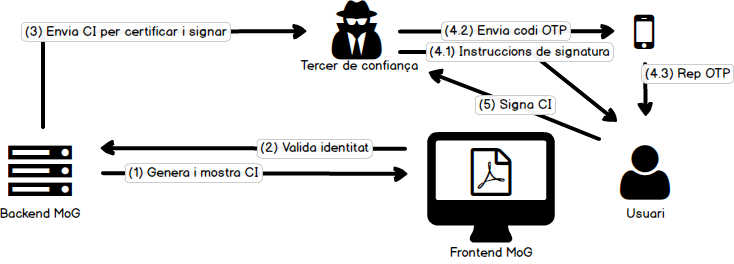
\includegraphics[scale=0.55]{sections/developement/trusted_thirdparty_arch.png}
\centering
\caption{Ús de tercers de confiança}
\label{fig:thirdparty_usage}
\end{figure}
\newline Veient la figura superior, ens n'adonem que les accions de pes recauen íntegrament sobre les espatlles del tercer de confiança, quedant per al projecte que aquí es desenvolupa les funcions d'interlocutor entre \textit{Lleida.net} i el \textit{backend}, i generar els consentiments informats.
\subsubsection{Generació de consentiments informats}
\begin{listing}[h]
\inputminted[
    firstline=74, 
    lastline=83,
    fontsize=\footnotesize]{php}{resources/src/InformedConsentGeneratorService.php}
\caption{Crida a la funció de renderitzat de Twig}
\label{code:twigRender}
\end{listing}
El fragment de codi anterior, mostra una crida a la llibreria de renderitzat de \textit{Symfony}\footnote{https://symfony.com/}. Juntament amb la llibreria \textit{wkhtmltopdf}\footnote{https://wkhtmltopdf.org/} es fan servir per, primerament, incrustar contingut dinàmicament a una plantilla HTML\footnote{HyperText Markup Language} i després, transformar aquest HTML en pdf mantenint els CSS\footnote{Cascading Style Sheets} de la plantilla.
\subsubsection{Funcionament del tercer de confiança i repercusions}
Tot i ser una dinàmica pròpia del tercer de confiança, és important conèixer el funcionament del servei que s'està a punt de fer servir.\\
\newline Com es pot veure a la Figura \ref{fig:thirdparty_usage}, el procés de certificació i posterior signatura segueixen una sèrie de passos estructurats i ben definits.
Un cop l'usuari ha validat la seva identitat, el \textit{backend} llança l'ordre de signatura del document que s'acaba de crear. Per això, s'envia un correu al tercer de confiança amb el document que es vol certificar i el destinatari (signant).\\
\newline Per la seva banda, \textit{Lleida.net}, en rebre l'ordre envia un segon correu a l'usuari amb:
\begin{itemize}
    \item Consentiment informat certificat.
    \item Instruccions per a la signatura.
    \item Enllaç a la web per signar el document.
\end{itemize}
Un cop l'usuari ha signat el document, \textit{Lleida.net} informa a l'emissor que la signatura del document s'ha dut a terme correctament.\\
\newline En aquest punt, on sembla ser que tot el procés s'ha dut a terme satisfactòriament, apareix el primer contratemps d'aquest projecte, i que provocarà un canvi d'estratègia global.\\
\newline \textit{Lleida.net} posa a disposició de l'emissor del document una plataforma des d'on recuperar els documents certificats.\\
\newline La impossibilitat d'automatitzar el procés obliga a recuperar de forma manual els documents, fet inadmissible ja que en termes d'escalabilitat, en el moment en que s'hagin de signar centenars de consentiments informats, amb la seva corresponent recuperació, el temps i l'esforç requerit seran massa grans.\\
Per tant, aquest fet obliga a descartar aquesta idea inicial.%ja que en el supòsit de que s'hagin de recuperar centenars de documents, com ja s'ha dit, s'hauria de fer manualment.

%\newline Com es pot veure, tota la activitat depèn íntegrament d'aquesta entitat externa. Un cop l'usuari ha validat la seva identitat com a signant, s'informa al tercer de confiança que ha d'iniciar el procés de signatura del document adjunt a l'ordre.\\
%\newline Aquest procés culmina amb un correu electrònic per part del tercer de confiança a l'usuari, on s'adjunta el consentiment informat certificat, unes instruccions a seguir per a signar el document i l'enllaç per a signar-lo.\\
%\newline La part fosca, i la que posa fi a la idea de fer ús dels serveis del tercer de confiança, és la manca d'una forma que es pugui automatitzar la recuperació dels documents certificats i signats. El tercer de confiança posa a disposició del seu client una plataforma que permet recuperar els resultats de les operacions que hagi dut a terme.